\documentclass[11pt]{article}
\usepackage[T1]{fontenc}
\usepackage[utf8]{inputenc}
\usepackage{lmodern}
\usepackage[a4paper,margin=2.5cm]{geometry}
\usepackage{amsmath,amssymb}
\usepackage{booktabs,multirow,tabularx,array}
\usepackage{graphicx}
\usepackage[font=small,labelfont=bf]{caption}
\usepackage{microtype}
\usepackage{enumitem}
\usepackage{authblk}
\usepackage{float}
\usepackage[section]{placeins}
\usepackage[numbers,sort&compress]{natbib}
\usepackage{xcolor}
\usepackage[colorlinks=true,allcolors=blue!50!black]{hyperref}
\usepackage{xurl}

\setlist{itemsep=2pt,topsep=4pt}
\setlength{\parskip}{0pt}
\renewcommand{\arraystretch}{1.1}
\newcommand{\AP}{\mathrm{AP}}
\newcommand{\LAT}{\mathrm{LAT}}

\title{Reconstructing 3D Bone Shapes from Biplanar X-rays:\\Three Deep Learning Models Tested on Six Datasets}

\author{}
\date{November 2026}

\begin{document}
\maketitle

\begin{abstract}
\noindent
A 3D model of a bone made from one front and one side X-ray image could help where CT is not available. The problem is hard because many different 3D shapes give the same two images, and published results are difficult to compare because studies use different bones and data. We trained three deep learning models under one protocol on six datasets built from TotalSegmentator, VerSe and CTPelvic1K: proximal femur, rib cage, two vertebra datasets and two pelvis datasets. The inputs are simulated X-ray images (digitally reconstructed radiographs) and the outputs are 3D bone masks. The models are a small two-view convolutional network (DualViewCNN), a multi-scale two-view network (MultiScale, 3.7M parameters) and Swin-X2S (Tiny version, 32.5M parameters, adapted from its official code). All three place the features of both views in 3D according to the X-ray geometry, which we checked with a projection test, and all were trained with the same epoch limit, batch size and early stopping. On 297 test cases, MultiScale had the highest mean Dice on all six datasets (femur 94.9\%, vertebrae 88.3\% and 89.2\%, pelvis 87.0\% and 86.6\%, rib cage 56.4\%), and SwinX2S was second on five. MultiScale's mean 95th-percentile Hausdorff distance was 2.4--5.2\,mm on all datasets except the rib cage (9.0\,mm). It scored higher than DualViewCNN on 296 of 297 cases and higher than SwinX2S on 282. After Holm correction, 11 of the 12 paired comparisons were significant; the exception was SwinX2S on VerSe20 ($n=10$). All inputs are simulated, and we did not measure clinical values. We release the trained models, per-case results and analysis scripts.
\end{abstract}

\noindent\textbf{Keywords:} biplanar X-ray, 3D bone reconstruction, digitally reconstructed radiographs, deep learning, Swin transformer, evaluation

% ======================================================================
\section{Introduction}

3D models of bones are used to plan orthopaedic surgery, to choose implant sizes and to measure deformities. They usually come from computed tomography (CT). CT costs more than plain X-ray imaging, is not available everywhere, and gives the patient a much higher radiation dose~\cite{brenner2007}. Biplanar radiography takes a front (anteroposterior, AP) image and a side (lateral) image of the same body region. It is cheap and common. Special low-dose systems that take both images at the same time are already used to build 3D models of the spine and legs by fitting shape models to the images~\cite{dubousset2005,humbert2009,melhem2016}.

Getting a 3D shape back from two projections is an ill-posed problem, because many different volumes give the same pair of images. Classical methods deal with this by using anatomical landmarks, bone outlines and statistical shape models, and they usually need some manual work~\cite{laporte2003,zheng2009,baka2011,karade2015}. Deep learning methods instead learn what bones look like from examples. Real paired data are rare, so these examples are usually made by computing simulated X-ray images, called digitally reconstructed radiographs (DRRs), from CT scans~\cite{ying2019,kasten2020,bayat2020,shakya2023,liuk2025}. An important design choice in these networks is how to place the features from the two 2D images into one 3D grid. The rays of the AP image go from front to back, and the rays of the lateral image go from side to side. One option is therefore to copy the features of each view along the direction of its rays, as in back-projection. Other designs let the network learn this mapping. Most studies test only one bone and use their own data splits, so it is hard to know how much such choices matter for different bones~\cite{shakya2023}.

In this paper we compare three models that we trained and tested with the same pipeline on six datasets from three public CT collections. The work started as an undergraduate project. The paper gives:
\begin{itemize}
\item test results for 18 models (three models on six datasets) trained under one protocol, with the same epoch limit, batch size and early stopping and with both views placed in 3D according to the X-ray geometry, tested once on held-out data, with per-case overlap and surface-distance scores and paired statistical tests;
\item the trained models, per-case test results, training logs and the scripts that make every table and figure.
\end{itemize}

We do not propose a new model. MultiScale follows the multi-scale two-view design in the benchmark of Shakya and Khanal~\cite{shakya2023}, which builds on X2CT-GAN~\cite{ying2019}. We wrote our own code for MultiScale and DualViewCNN. For SwinX2S we started from the official code of Swin-X2S~\cite{liuk2025} and changed some parts of it (Section~\ref{sec:models}). All inputs are simulated X-ray images and we did not measure clinical values. Our results therefore show how well the predicted shapes match the true shapes on simulated data. They do not show clinical accuracy.

% ======================================================================
\section{Related Work}

\paragraph{Classical biplanar reconstruction.}
Landmark-based methods find anatomical points in two calibrated X-ray images and compute their 3D positions, for example with the direct linear transformation. This gives only a small number of 3D points~\cite{zhang2010}. Contour-based methods match the bone outlines in the two images to a 3D model~\cite{laporte2003}. Template-based methods deform a general bone model until its projections fit the outlines in the images~\cite{gunay2007}, for example with Laplacian surface deformation~\cite{karade2015}. Statistical shape models describe how bone shapes vary between people~\cite{heimann2009}. They make the fit more reliable when the outlines are incomplete or noisy~\cite{zheng2009,baka2011}. Shape models of this kind are used in clinical 3D reconstruction of the spine from low-dose biplanar systems~\cite{humbert2009,melhem2016}. These methods need calibrated images and bone outlines, often with manual input, and their accuracy depends on how well the template or shape model fits the patient.

\paragraph{Learning-based reconstruction.}
X2CT-GAN reconstructs CT volumes from two X-ray images taken at right angles, using a generative adversarial network~\cite{ying2019}. Single-view methods recover volumes or surfaces from only one image and depend on strong learned priors~\cite{henzler2018,shen2019,gu2024}. For bones, Kasten et al.\ reconstruct knee bones from two X-ray images with a CNN trained on DRRs~\cite{kasten2020}. Bayat et al.\ estimate the 3D posture of the spine from two X-ray images~\cite{bayat2020}, and Shiode et al.\ reconstruct the forearm bones near the wrist from real X-ray images~\cite{shiode2021}. Shakya and Khanal compare several encoder--decoder models on four anatomies with one shared pipeline, including models that combine the two views at several resolutions, and they propose clinical measures for each anatomy~\cite{shakya2023}. Swin-X2S uses a 2D Swin transformer encoder~\cite{swin2021}, a module that places coronal and sagittal features along different axes of the volume, cross-attention between the views, and a 3D convolutional decoder~\cite{liuk2025}. Sparse-view X-ray methods based on radiance fields or similar learned volume representations~\cite{cai2024,wang2025xfield} solve a related but different problem. They recover attenuation volumes from several projections, not bone shapes from two.

\paragraph{Simulated X-ray images and datasets.}
Public datasets with paired X-ray images and CT scans are rare. Most deep learning work therefore trains on DRRs, which are made by casting rays through CT volumes~\cite{siddon1985,ehlke2013}. DRRs have no scatter, no detector noise and none of the changes in patient position seen in real images, so results on DRRs may not carry over to real X-ray images~\cite{shakya2023}. The CT collections we use, TotalSegmentator~\cite{wasserthal2023}, VerSe~\cite{verse2021} and CTPelvic1K~\cite{pelvic2020}, come with bone labels, and our target masks are made from these labels.

\paragraph{Evaluation.}
Overlap scores such as Dice are standard, but they change little when there are errors at the border of a large structure. For this reason they are usually reported together with surface distances~\cite{taha2015,maierhein2024}. The normalized surface Dice measures how much of the surface lies within a set distance (the tolerance) of the true surface~\cite{nikolov2021}.

% ======================================================================
\section{Materials and Methods}\label{sec:methods}

\begin{figure}[t]
\centering
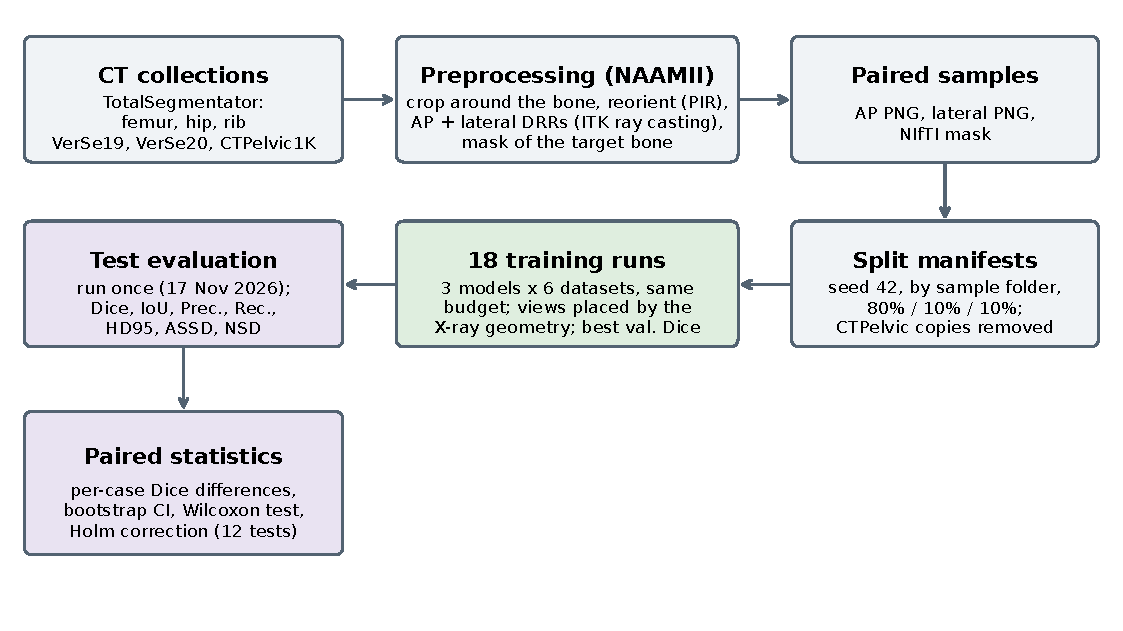
\includegraphics[width=0.92\textwidth]{figures/overview.pdf}
\caption{Overview of the study. NAAMII prepared the data. We made the splits, trained the 18 models, tested them once on the test splits.}
\label{fig:overview}
\end{figure}

\subsection{Problem setup}\label{sec:problem}
Each sample has an AP image $X_\AP$, a lateral image $X_\LAT$ and a binary mask $Y$ of one bone or group of bones. All three come from the same region of one CT scan. Volumes are stored as arrays with indices $(d,h,w)$ that increase towards posterior, inferior and right (PIR in the nibabel convention). So the first axis ($D$) runs from front to back, the second ($H$) from head to feet, and the third ($W$) from left to right. The rays of the AP image travel along $D$, and the rays of the lateral image travel along $W$. In the stored images, rows follow $H$ and the columns of the lateral image follow $D$ in the same direction. The columns of the stored AP image run opposite to $W$. This is the usual way X-ray images are displayed, with the patient's right side on the left of the image. We therefore mirror every AP image left to right when it is loaded. After this, for an ideal parallel-beam projection of a quantity $f$ that adds up along the ray,
\begin{equation}
X_\AP(h,w)\propto\sum_{d} f(d,h,w),\qquad X_\LAT(h,d)\propto\sum_{w} f(d,h,w).
\label{eq:projection}
\end{equation}
We checked these directions on every sample by correlating the loaded images with projections of their masks. After the AP mirroring, the AP image matched the projection better than its mirror image in 96.9--100\% of the samples of each dataset. The lateral image matched in 99.5--100\% of the samples of femur, hip, rib and CTPelvic, and in 81\% (VerSe19) and 91\% (VerSe20) of the vertebra samples. For single vertebrae the correlations are low overall, because the images also show the neighbouring vertebrae; in the mismatched cases the two correlations were nearly equal, and visual checks of such cases showed the expected orientation.
A model $g_\theta$ takes the two images and predicts a probability for every voxel, $\hat Y=g_\theta(X_\AP,X_\LAT)\in[0,1]^{D\times H\times W}$. We threshold these probabilities at 0.5 to get the predicted mask.

\subsection{Datasets}\label{sec:data}
Figure~\ref{fig:overview} gives an overview of the study. We use six datasets (Table~\ref{tab:data}). NAAMII provided the processed DRRs and masks. They were made with NAAMII's open-source XrayTo3DPreprocess pipeline~\cite{xrayto3dpreprocess}, which is the data pipeline of the benchmark of Shakya and Khanal~\cite{shakya2023}. The pipeline cuts a box of fixed physical size from each CT scan at the scan's own voxel spacing, turns it to the PIR orientation, keeps the target label inside the box as the mask, and computes the two DRRs from this box (Section~\ref{sec:drr}). What one sample contains is different for each dataset:
\begin{itemize}
\item \textbf{Femur} (TotalSegmentator~\cite{wasserthal2023}): the upper (proximal) femur in a 128\,mm box whose top edge is just above the femoral head, so the box cuts through the shaft. Left femurs and mirrored right femurs are separate samples (376 left, 368 right). The mask is the largest connected part of the femur label.
\item \textbf{Hip} (TotalSegmentator): both hip bones and the sacrum in a 288\,mm box centred on the mask's centre of mass, one sample per CT.
\item \textbf{Rib} (TotalSegmentator): all 24 ribs together in a 320\,mm box centred on the mask's centre of mass, one sample per CT with a complete rib cage.
\item \textbf{VerSe19} and \textbf{VerSe20} (VerSe~\cite{verse2021}): one vertebra per sample in a 96\,mm box around the vertebra centre given with VerSe. For VerSe20 the box is shifted so that 70\% of it lies behind (posterior to) the centre.
\item \textbf{CTPelvic} (CTPelvic1K~\cite{pelvic2020}, CT colonography subset): both hip bones and the sacrum in a 288\,mm box, one sample per CT.
\end{itemize}
Hip and CTPelvic therefore have the same target but come from different CT collections. The TotalSegmentator masks have 1.5\,mm voxels in every direction. The VerSe and CTPelvic masks keep the uneven (anisotropic) voxel spacing of the original scans. Because the boxes have a fixed size, many masks are cut off at the box faces. We checked 80 masks per dataset (27 for VerSe20). All femur masks touched at least one face of the box, and so did 45 hip, 65 rib, 29 CTPelvic, 46 VerSe19 and 6 VerSe20 masks. The task is to reconstruct the part of the bone that lies inside the box.

\begin{table}[t]
\centering
\caption{Datasets, splits and output grids. Counts are samples: one femur side, one vertebra, or one CT for hip, rib and CTPelvic. The voxel size is that of the output grid on which the models are trained and tested.}
\label{tab:data}
\small
\begin{tabular}{lrrrrcc}
\toprule
Dataset & Train & Val. & Test & Total & Grid $(D,H,W)$ & Voxel (mm) \\
\midrule
Femur & 595 & 74 & 75 & 744 & $96\times96\times128$ & $1.33\times1.33\times1.00$ \\
Hip & 285 & 36 & 35 & 356 & $128\times128\times160$ & $2.25\times2.25\times1.80$ \\
Rib & 307 & 38 & 39 & 384 & $128\times128\times160$ & $2.50\times2.50\times2.00$ \\
VerSe19 & 747 & 93 & 94 & 934 & $96\times96\times128$ & $1.00\times1.00\times0.75$ \\
VerSe20 & 85 & 11 & 10 & 106 & $96\times96\times128$ & $1.00\times1.00\times0.75$ \\
CTPelvic & 412 & 48 & 44 & 504 & $128\times128\times160$ & $2.25\times2.25\times1.80$ \\
\bottomrule
\end{tabular}

\end{table}

\subsection{Simulated X-ray images}\label{sec:drr}
By the Beer--Lambert law, the intensity behind an object is $I=I_0\exp\!\left(-\int_{r}\mu(\mathbf{x})\,\mathrm{d}l\right)$, where $\mu$ is the linear attenuation coefficient along the ray $r$. The log image $-\ln(I/I_0)$ is therefore a line integral of $\mu$. DRRs imitate this by casting rays through a CT volume~\cite{siddon1985}. Our DRRs were computed with the ray caster in ITK's TwoProjectionRegistration module (\texttt{GetDRRSiddonJacobsRayTracing}), which is based on Siddon's algorithm, using the settings of the XrayTo3DPreprocess pipeline. The source is 1000\,mm from the centre of the box. The image plane passes through the centre of the box and has 1\,mm pixels. The image size in pixels equals the box size in millimetres (128 for femur, 288 for hip and CTPelvic, 320 for rib and 96 for the vertebrae). Each pixel value is
\begin{equation}
P(u,v)=\frac{1}{\lVert \mathbf{p}_{uv}-\mathbf{s}\rVert}\int_{r(u,v)}\max\bigl(\mathrm{HU}(\mathbf{x})-\tau,\,0\bigr)\,\mathrm{d}l,\qquad \tau=0\ \mathrm{HU},
\label{eq:drr}
\end{equation}
where $\mathbf{s}$ is the source and $\mathbf{p}_{uv}$ is the pixel position. This is a plain line integral of the thresholded CT values, with no exponential. The images therefore look like log-transformed X-ray images in which only tissue above 0\,HU is visible. Each image is stored as a 16-bit integer, scaled from its own minimum and maximum to 8 bits, and saved as a PNG. Only the box is projected, so anatomy outside the box does not appear in the images. With the source at 1000\,mm, the rays at the edges of the widest images (rib) are tilted by about $9^\circ$, so Equation~\eqref{eq:projection} is only approximately true. We also wrote a separate C++ DRR renderer (Appendix~\ref{app:renderer}). It was not used to make the data for the experiments in this paper.

\subsection{Data splits}\label{sec:splits}
The processed data came with training, validation and test folders, but the validation and test folders were subsets of the training folder. We therefore did not use them. Instead, we split all sample folders of each dataset once, with random seed 42, into 80\% training, 10\% validation and 10\% test samples. A sample was kept only if both images and the mask were present. All three models use the same splits. No sample ID appears in two splits, and the test split was not used for training, early stopping or choosing checkpoints. In CTPelvic, 37 scans were stored twice under different folder names, with identical images and masks. We kept one copy of each: the copy in the training split if there was one, otherwise the one in the validation split. This leaves 412 training, 48 validation and 44 test samples, with no scan in more than one split.

The splits are made by sample folder, and the folders do not record which scan or person a sample came from. This has two effects. First, each VerSe sample is a single vertebra, so vertebrae from the same scan can end up in different splits. Second, the two femurs of one TotalSegmentator scan are separate samples and look alike after mirroring. With random splitting, about a third of the scans that give both femurs would have them in different splits. We tried to find these pairs by crop position and by image similarity, but we could not tell them apart from unrelated femurs, so we do not know how often this happened. Section~\ref{sec:limitations} discusses the effect of these issues.

\subsection{Preprocessing and augmentation}\label{sec:preproc}
Both images are turned into single-channel tensors with values in $[0,1]$, the AP image is mirrored left to right (Section~\ref{sec:problem}), and both are resized with antialiasing to $H\times W$, the in-plane size of the output grid. For the lateral image, this means that the horizontal axis, which belongs to $D$, is resampled to $W$ pixels. All three models resample it back to $D$ when they place the lateral features in the volume. The mask is scaled to $[0,1]$ by its minimum and maximum and resized to $(D,H,W)$ with trilinear interpolation. This resized mask, which has values between 0 and 1 at the border, is the training target. For evaluation it is thresholded at 0.5. Table~\ref{tab:data} lists the grids and voxel sizes.

During training only, we use three flips, each with probability 0.5, applied to the images and the mask together: head--feet (both images and the volume), left--right (the AP image and the volume) and front--back (the lateral image and the volume). Then, with probability 0.8, each image gets a random gamma change in $[0.85,1.15]$, a gain in $[0.90,1.10]$, an offset in $[-0.05,0.05]$ and Gaussian noise with standard deviation 0.02, and is clipped to $[0,1]$. We did not use rotations, crops or shifts. Applying them to the images without the same 3D change to the mask would break the match between the inputs and the target.

\subsection{Models}\label{sec:models}

\paragraph{Placing 2D features in the volume.}
From Equation~\eqref{eq:projection}, a feature map $A\in\mathbb{R}^{C\times H\times W}$ from the (mirrored) AP image and a feature map $B\in\mathbb{R}^{C\times H\times D}$ from the lateral image can be placed in the volume in a way that matches the geometry by copying each one along its ray direction:
\begin{equation}
\mathcal{L}_\AP(A)[c,d,h,w]=A[c,h,w],\qquad \mathcal{L}_\LAT(B)[c,d,h,w]=B[c,h,d].
\label{eq:lifting}
\end{equation}
This is the simple (unweighted) back-projection of each view. All three models place the two views along these axes, either by copying (MultiScale) or by a learned expansion along the ray direction (DualViewCNN, SwinX2S). We checked this for every model with a sensitivity test: with random weights, a small bright square was moved across the columns of one input image, and we recorded where the output changed. For every model, moving the square across the AP image moved the change along $W$, and moving it across the lateral image moved the change along $D$, in the same direction (correlation above 0.99), while the position along the other axis stayed fixed.

\paragraph{DualViewCNN.}
DualViewCNN is a small baseline that we wrote for this project (Fig.~\ref{fig:dualview}). Its two-view layout follows the `map \& fuse' design of TransVert~\cite{bayat2020}, a fully convolutional network that encodes each view in 2D, expands it into 3D and fuses the two views before a 3D decoder. Unlike TransVert, DualViewCNN has no vertebra-annotation input and no attention layer. Each view has its own encoder of two strided $3\times3$ convolutions. These reduce the image to a thin slab of 32 feature channels (48 for rib) at a quarter of the input resolution. Transposed convolutions with stride 2 along one axis grow each slab to a quarter of the target depth, followed by two $3\times3\times3$ convolutions. The two volumes are joined (concatenated) and decoded by two transposed $4\times4\times4$ convolutions with stride 2 and two more convolutions, with group normalization (8 groups)~\cite{wu2018}, which does not depend on the batch size. The AP slab is grown along $D$. For the lateral slab, the horizontal axis of the lateral image is first resized to the depth of the volume and placed on $D$, and the slab is then grown along $W$, the direction of the lateral rays. DualViewCNN has 564,321 parameters on the $96\times96\times128$ grids, 566,465 on the hip and CTPelvic grids and 1,264,993 in the wider rib version.

\paragraph{MultiScale.}
MultiScale (Fig.~\ref{fig:multiscale}) gives each view its own 2D encoder with four residual stages~\cite{he2016} of 16, 32, 64 and 128 channels (stride 1 in the first stage and 2 in the others), and its own 2D decoder with skip connections~\cite{ronneberger2015}. At each of the four decoder scales $s$, from coarse to fine, the decoded features $A_s$ and $B_s$ are resized to the in-plane size of that scale and copied into the volume:
\begin{equation}
Z_s=R_s\!\left(\left[\,\mathcal{U}(Z_{s-1}),\ \mathcal{L}_\AP(A_s),\ \mathcal{L}_\LAT(B_s)\,\right]\right).
\label{eq:multiscale}
\end{equation}
Here $[\cdot]$ means joining along the channel axis, $\mathcal{U}$ is trilinear upsampling, and $R_s$ is a residual block of two $3\times3\times3$ convolutions with group normalization~\cite{wu2018}. The coarsest scale, at 1/8 of the output size, has no $Z_{s-1}$. The finest scale has the full output size. A final $1\times1\times1$ convolution gives the output logits. MultiScale has 3,730,033 parameters. It follows the multi-scale two-view design in the benchmark of Shakya and Khanal~\cite{shakya2023}, but we wrote the code ourselves and did not use theirs.

\paragraph{SwinX2S.}
SwinX2S (Fig.~\ref{fig:swin}) is the Swin-X2S model of Liu et al.~\cite{liuk2025}. We started from their official code, which is released under the MIT licence, and changed a few parts of it to fit our pipeline. One 2D Swin transformer~\cite{swin2021} with patch size 2, $7\times7$ windows and depths $(2,2,6,2)$ encodes both views with shared weights. As in the official code, it uses stochastic depth (drop path) with a rate rising to 0.2. At each of six levels (the input and five feature resolutions), a $1\times1\times1$ convolution turns the 2D feature map into a volume by expanding a singleton axis; it is initialized to copy the features. In the official code, the volumes of the two views are then arranged along different axes~\cite[Sec.~3.2]{liuk2025}, for that code's own image layout. We arranged them for our layout (Equation~\ref{eq:lifting}): the AP features are expanded along $D$, and for the lateral features the horizontal image axis is resized to the depth of that level, placed on $D$ and expanded along $W$ by a second set of $1\times1\times1$ convolutions. Residual 3D blocks with shared weights then process the volumes of each view. At the coarsest level (1/32 of the output size), one cross-view attention block passes information between the views:
\begin{equation}
\mathrm{CrossAttn}(Q_i,K_j,V_j)=\operatorname{softmax}\!\left(\frac{Q_iK_j^{\top}}{\sqrt{d_k}}\right)V_j,\qquad (i,j)\in\{(\AP,\LAT),(\LAT,\AP)\}.
\label{eq:attention}
\end{equation}
The queries come from one view and the keys and values from the other. They are computed after layer normalization and with a shared learned position embedding. As in the official code, the attention output replaces the bottleneck features, and there is no feed-forward layer and no residual connection. A shared 3D decoder with five upsampling stages and skip connections gives one output volume per view. As in the official code, the prediction is the mean of the two output logits, and training uses the official two-output loss: for each output, the segmentation loss (Equation~\ref{eq:loss}) plus the Kullback--Leibler divergence from the other output's predicted probabilities, averaged over the two outputs. We use the Tiny version on all datasets (embedding dimension 32, heads $(1,2,4,8)$, one attention layer) with instance normalization in the 3D blocks, the default of the official model. It has 32,533,905 parameters on the $96\times96\times128$ grids and 32,556,749 on the $128\times128\times160$ grids.

\begin{figure}[t]
\centering
\begin{minipage}[t]{0.47\textwidth}\centering
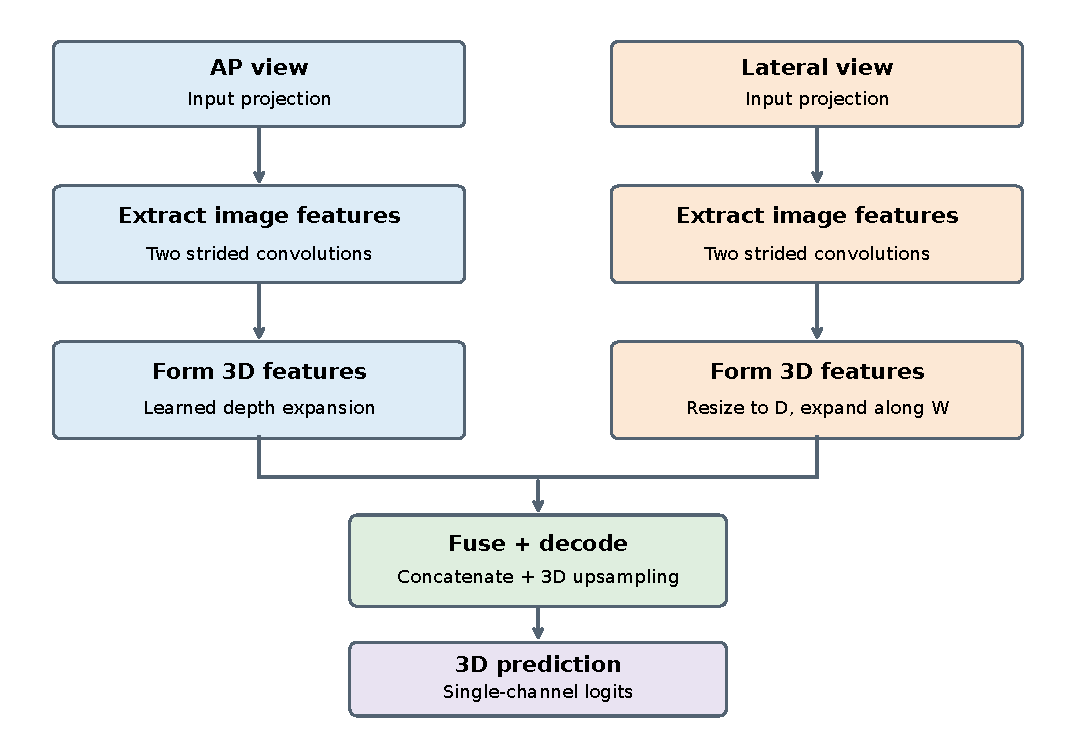
\includegraphics[width=\textwidth]{figures/cnn_dualview_architecture.pdf}
\caption{DualViewCNN. Each view has its own encoder, which gives a thin slab of features. The AP slab is grown along $D$; the lateral slab is resized to the depth of the volume and grown along $W$. The two volumes are joined and decoded in 3D.}
\label{fig:dualview}
\end{minipage}\hfill
\begin{minipage}[t]{0.49\textwidth}\centering
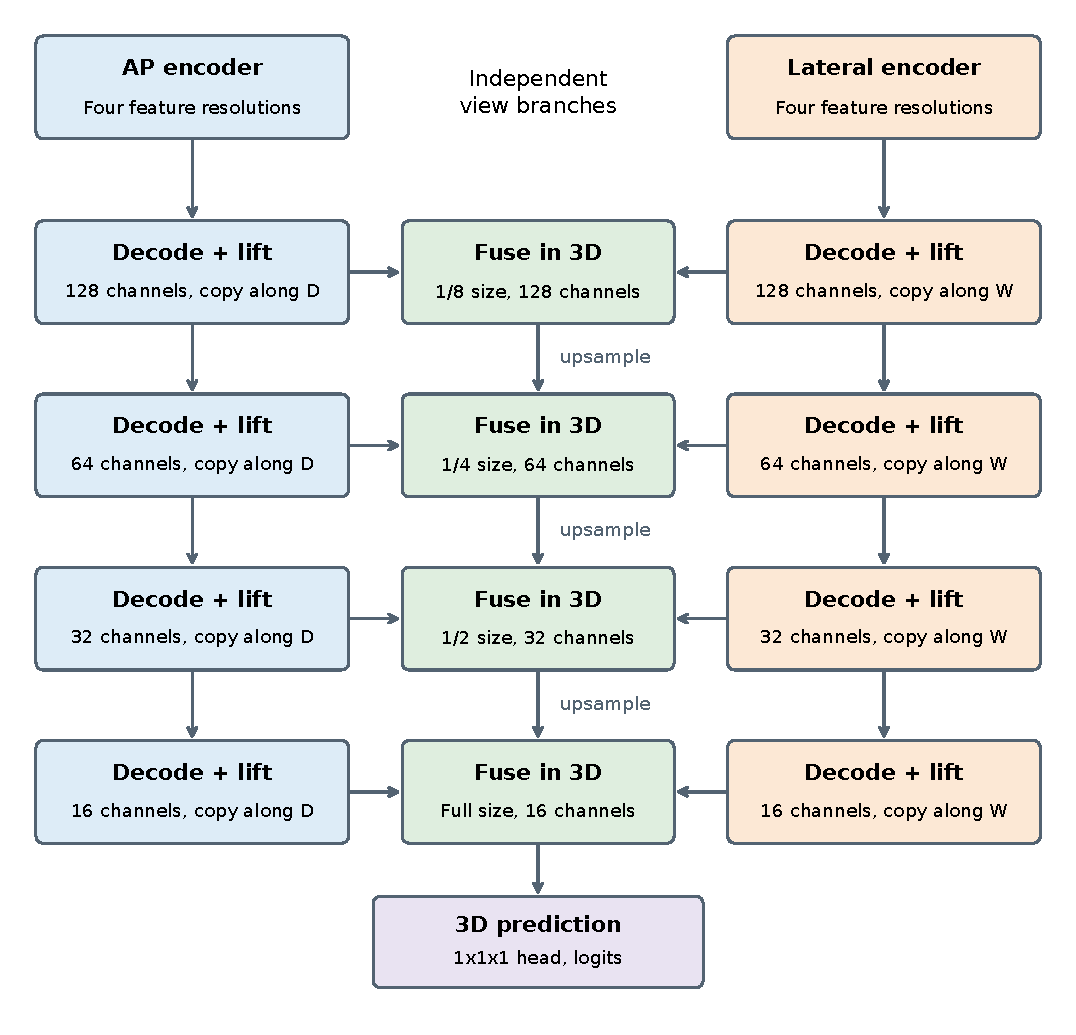
\includegraphics[width=\textwidth]{figures/cnn_multiscale_architecture.pdf}
\caption{MultiScale, from coarse to fine. Each side branch decodes one view and copies its features into 3D (Equation~\ref{eq:multiscale}). Each fusion block joins the two views with the upsampled volume from the previous scale and applies a residual 3D block. Skip connections from the encoders are not shown.}
\label{fig:multiscale}
\end{minipage}
\end{figure}

\begin{figure}[t]
\centering
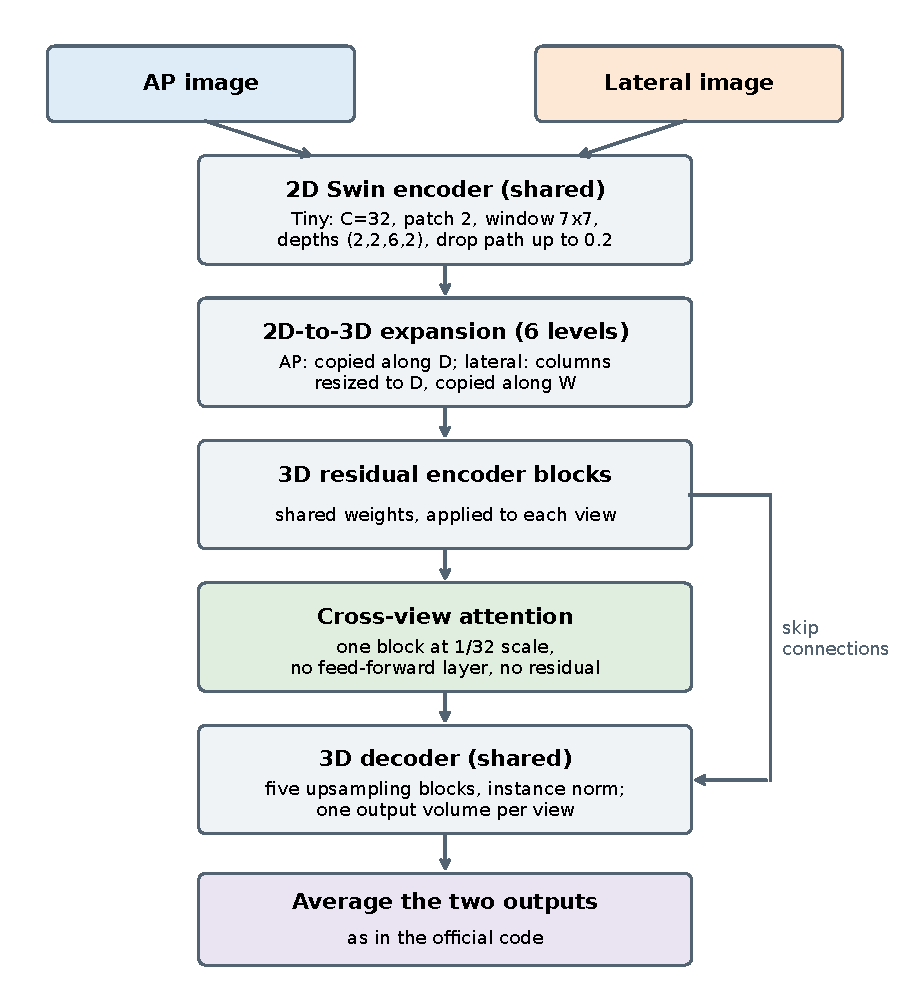
\includegraphics[width=0.5\textwidth]{figures/swinx2s_implementation.pdf}
\caption{SwinX2S as used in this paper, adapted from the official Swin-X2S code~\cite{liuk2025}. The encoder, 3D blocks and decoder are shared by the two views. The expansion step places the AP features along $D$ and the lateral features along $W$ (Equation~\ref{eq:lifting}), and the two output volumes are averaged.}
\label{fig:swin}
\end{figure}

\begin{table}[t]
\centering
\caption{The three models as built and trained.}
\label{tab:models}
\small
\begin{tabularx}{\textwidth}{@{}>{\raggedright\arraybackslash}p{0.18\textwidth}*{3}{>{\raggedright\arraybackslash}X}@{}}
\toprule
 & DualViewCNN & MultiScale & SwinX2S \\
\midrule
2D encoder & two strided convolutions per view & four residual stages per view, with 2D decoder & one Swin transformer (Tiny) shared by both views \\
2D to 3D (Eq.~\ref{eq:lifting}) & learned expansion along $D$ (AP) and $W$ (lateral) & copying along $D$ (AP) and $W$ (lateral) at four scales & $1\times1\times1$ expansion along $D$ (AP) and $W$ (lateral), six levels \\
View fusion & concatenation, once & concatenation at four scales & cross-attention at 1/32 scale; the two outputs are averaged \\
Normalization & group & group & instance (layer norm in transformer) \\
Parameters & 0.56M (rib: 1.26M) & 3.73M & 32.5M \\
\bottomrule
\end{tabularx}
\end{table}

% ======================================================================
\section{Experimental Setup}\label{sec:setup}

\subsection{Training}
All models were written in PyTorch and trained with an equal mix of binary cross-entropy and soft Dice loss~\cite{milletari2016}:
\begin{equation}
\mathcal{L}=\tfrac12\,\mathcal{L}_{\mathrm{BCE}}+\tfrac12\left(1-\frac{1}{B}\sum_{b=1}^{B}\frac{2\sum_v p_{bv}y_{bv}+1}{\sum_v p_{bv}+\sum_v y_{bv}+1}\right),
\label{eq:loss}
\end{equation}
where $p_{bv}$ is the predicted probability and $y_{bv}$ the target value of voxel $v$ in sample $b$ of a batch of size $B$ (for SwinX2S, the two-output form described in Section~\ref{sec:models}). All runs used random seed 42, cuDNN in deterministic mode, automatic mixed precision~\cite{micikevicius2018} and gradient clipping at a global norm of 1. Even so, the runs cannot be repeated bit for bit, because some CUDA operations used in training are not deterministic. Table~\ref{tab:training} gives the optimization settings. All models share the epoch limit (200), the batch size (2), early stopping after 40 epochs without a better validation Dice, the augmentation and the loss. Each model keeps the optimizer, learning rate and schedule of its original setting; we did not tune these. SwinX2S was trained from random starting weights, without pretraining. For every run we kept the weights from the epoch with the highest mean validation Dice.

Fourteen runs were trained on one NVIDIA GeForce RTX 5090 GPU. SwinX2S on hip, rib, CTPelvic and VerSe20 was trained on NVIDIA L40S GPUs of a cloud service, with a time limit per run. Two of these runs reached the limit before epoch 200: hip stopped after epoch 195 and CTPelvic after epoch 190, when the cosine schedule had already lowered the learning rate below $10^{-6}$. Their best epochs were 171 and 169. The CTPelvic run was interrupted once by the cloud service (preemption) and restarted from the beginning; only the complete restarted run is used.

\begin{table}[t]
\centering
\caption{Training settings. For the CNNs, the learning rate is halved after 10 epochs without a lower validation loss. SwinX2S uses a 20-epoch linear warm-up followed by cosine decay over the 200 epochs. Early stopping counts epochs without a better validation Dice.}
\label{tab:training}
\small
\begin{tabular}{@{}lccc@{}}
\toprule
 & DualViewCNN & MultiScale & SwinX2S \\
\midrule
Optimizer & Adam & Adam & AdamW, weight decay 0.05 \\
Initial learning rate & $1\times10^{-4}$ & $2\times10^{-4}$ & $3\times10^{-5}$ \\
Schedule & reduce on plateau & reduce on plateau & warm-up, cosine \\
Maximum epochs & 200 & 200 & 200 \\
Early stopping & 40 epochs & 40 epochs & 40 epochs \\
Batch size & 2 & 2 & 2 \\
\bottomrule
\end{tabular}
\end{table}

\subsection{Evaluation protocol}
We trained all 18 models and chose their checkpoints on the validation splits before we used the test splits. No model or training setting was chosen using test results. As a check, the evaluation code first scored the validation splits again and matched the validation Dice stored with each checkpoint to within $1.1\times10^{-5}$ for all 18 runs. We then scored the test splits once, on 17 November 2026.

\subsection{Metrics}
Predictions and targets are thresholded at 0.5 on the output grid. With $TP$, $FP$ and $FN$ the numbers of true-positive, false-positive and false-negative voxels, we compute
\begin{align}
\mathrm{Dice}&=\frac{2TP}{2TP+FP+FN}, & \mathrm{IoU}&=\frac{TP}{TP+FP+FN},\nonumber\\
\mathrm{Prec.}&=\frac{TP}{TP+FP}, & \mathrm{Rec.}&=\frac{TP}{TP+FN}.
\end{align}
For the surface metrics, let $S_P$ and $S_G$ be the boundary voxels of the predicted and true masks, that is, mask voxels with at least one 6-connected neighbour outside the mask. Let $d(x,S)$ be the Euclidean distance in millimetres from voxel $x$ to the nearest voxel of $S$. We compute it with an exact distance transform that uses the real (anisotropic) voxel size of the grid. Then
\begin{align}
\mathrm{HD95}&=\max\Bigl(\mathrm{P}_{95}\{d(x,S_G)\}_{x\in S_P},\ \mathrm{P}_{95}\{d(y,S_P)\}_{y\in S_G}\Bigr),\\
\mathrm{ASSD}&=\frac{\sum_{x\in S_P}d(x,S_G)+\sum_{y\in S_G}d(y,S_P)}{|S_P|+|S_G|},\\
\mathrm{NSD}_\tau&=\frac{|\{x\in S_P:d(x,S_G)\le\tau\}|+|\{y\in S_G:d(y,S_P)\le\tau\}|}{|S_P|+|S_G|},\qquad\tau=1.5\ \mathrm{mm},
\end{align}
where $\mathrm{P}_{95}$ is the 95th percentile. Our NSD is a voxel-based version of the normalized surface Dice~\cite{nikolov2021}, and the 1.5\,mm tolerance follows~\cite{shakya2023}. Voxels on the faces of the box count as boundary voxels, so masks cut by the box add flat, artificial surfaces to both the prediction and the reference. No model gave an empty prediction for any test case, so every metric is defined for every case. We report means over test cases, standard deviations for Dice, and for HD95 also the median, because a few cases with far-away false-positive pieces can raise the mean a lot.

Two things about these metrics matter when reading the results. First, the output grids are coarse (Table~\ref{tab:data}). Voxels are 1.0--1.33\,mm along $D$ and $H$ (0.75--1.0\,mm along $W$) for femur and the vertebrae, and 2.25--2.5\,mm along $D$ and $H$ (1.8--2.0\,mm along $W$) for hip, CTPelvic and rib. Surface errors smaller than about one voxel cannot be measured. On hip, CTPelvic and rib the 1.5\,mm NSD tolerance is smaller than a voxel, which makes NSD very strict there. Second, Dice depends on the size and shape of the structure. A one-voxel error lowers Dice much more for thin ribs or a small vertebra than for the femur. We therefore use Dice to compare models on the same dataset, not to rank anatomies.

\subsection{Statistical analysis}
To compare MultiScale with each of the other two models, we use the per-case difference in Dice on the same test cases. We report the mean difference with a 95\% percentile bootstrap confidence interval (10,000 resamples), the number of cases in which MultiScale scores higher, and a two-sided Wilcoxon signed-rank test~\cite{wilcoxon1945}. The test uses the exact distribution for $n\le50$ and a normal approximation otherwise, as in SciPy~1.18. We adjust the $p$-values of the 12 comparisons (two per dataset) with the Holm method~\cite{holm1979} and call a difference significant if the adjusted $p$-value is below 0.05. As an exploratory analysis, we compare SwinX2S with DualViewCNN in the same way, with a separate Holm correction over its six tests. The bootstrap uses a fixed random seed (0). With only 10 cases (VerSe20), the bootstrap interval is only approximate. These tests assume that test cases are independent. This is not fully true for VerSe, where several vertebrae can come from one scan, or for femur, where two femurs can come from one scan. The tests also do not cover the variation between training runs, because we trained each model only once.

% ======================================================================
\section{Results}\label{sec:results}

\subsection{Overall test results}
Table~\ref{tab:test} gives the mean test Dice of the 18 models, and Fig.~\ref{fig:box} shows the score of every test case. MultiScale has the highest mean Dice on every dataset: 94.9\% on femur, 88.3\% and 89.2\% on VerSe19 and VerSe20, 87.0\% on hip, 86.6\% on CTPelvic and 56.4\% on rib. SwinX2S is second on five datasets (93.6\%, 85.5\%, 88.3\%, 84.7\% and 82.4\%), and DualViewCNN is second on rib (47.5\% against 45.4\% for SwinX2S). Averaged over the six datasets, the mean Dice is 83.7\% for MultiScale, 80.0\% for SwinX2S and 72.6\% for DualViewCNN. For all 18 runs, the test Dice is between 1.2 points below and 3.9 points above the validation Dice of the chosen checkpoint (Appendix~\ref{app:training}).

\begin{table}[t]
\centering
\caption{Test Dice (\%, mean $\pm$ standard deviation over the $n$ test cases). The best model for each dataset is in bold.}
\label{tab:test}
\small
\begin{tabular}{lrccc}
\toprule
Dataset & $n$ & DualViewCNN & MultiScale & SwinX2S \\
\midrule
Femur & 75 & 92.5 $\pm$ 4.7 & \textbf{94.9 $\pm$ 2.6} & 93.6 $\pm$ 3.5 \\
Hip & 35 & 80.8 $\pm$ 4.1 & \textbf{87.0 $\pm$ 2.7} & 84.7 $\pm$ 2.5 \\
Rib & 39 & 47.5 $\pm$ 10.0 & \textbf{56.4 $\pm$ 9.7} & 45.4 $\pm$ 11.2 \\
VerSe19 & 94 & 66.5 $\pm$ 18.1 & \textbf{88.3 $\pm$ 5.2} & 85.5 $\pm$ 6.4 \\
VerSe20 & 10 & 69.4 $\pm$ 21.7 & \textbf{89.2 $\pm$ 3.7} & 88.3 $\pm$ 2.4 \\
CTPelvic & 44 & 79.0 $\pm$ 4.2 & \textbf{86.6 $\pm$ 2.5} & 82.4 $\pm$ 3.2 \\
\bottomrule
\end{tabular}

\end{table}

\begin{figure}[t]
\centering
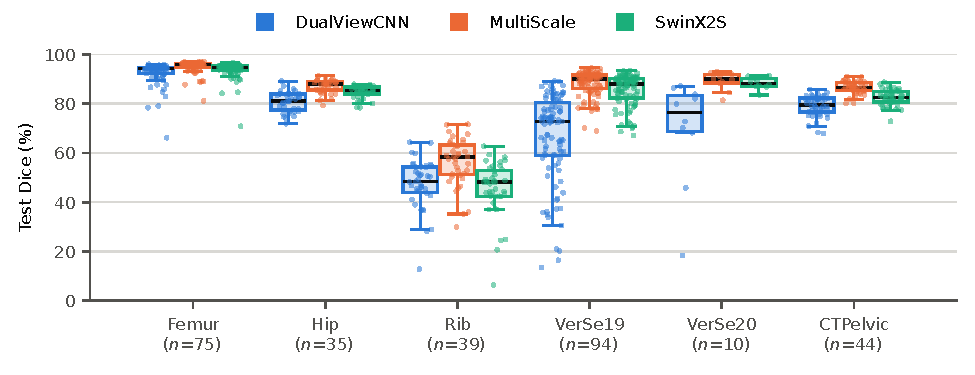
\includegraphics[width=\textwidth]{figures/test_dice_distribution.pdf}
\caption{Test Dice of every case. Boxes show the interquartile range and median, whiskers reach at most 1.5 times the interquartile range, and dots are single test cases. CTPelvic shows 44 test cases.}
\label{fig:box}
\end{figure}

The case-by-case comparison (Table~\ref{tab:paired}) shows that the ranking holds for most cases. MultiScale scores higher than DualViewCNN on 296 of 297 test cases, with mean differences from 2.5 points (femur) to 21.8 points (VerSe19). It scores higher than SwinX2S on 282 of 297 cases, with mean differences from 0.9 points (VerSe20) to 11.0 points (rib); on femur, hip, VerSe19 and CTPelvic the difference is 1.3 to 4.1 points. All differences are significant after Holm correction except MultiScale against SwinX2S on VerSe20 (adjusted $p=0.28$). This dataset has only 10 test cases, MultiScale is better on 8 of them, and the confidence interval of the mean difference includes zero ($-0.2$ to $+1.8$ points). We therefore do not conclude that MultiScale is better than SwinX2S on VerSe20. In the exploratory comparison, SwinX2S scores higher than DualViewCNN on five datasets (by 1.2 to 19.1 points, all significant after Holm correction) and lower on rib, by 2.1 points (95\% CI $-3.4$ to $-0.9$; adjusted $p=0.004$).

\begin{table}[t]
\centering
\caption{Paired test comparison of MultiScale with the other two models. $\Delta$Dice: mean per-case difference in Dice points, with a 95\% bootstrap confidence interval. Wins: test cases in which MultiScale scores higher. $p_{\rm Holm}$: two-sided Wilcoxon signed-rank test, Holm-adjusted over the 12 comparisons.}
\label{tab:paired}
\small
\setlength{\tabcolsep}{5pt}
\begin{tabular}{lrrrrrr}
\toprule
& \multicolumn{3}{c}{MultiScale $-$ DualViewCNN} & \multicolumn{3}{c}{MultiScale $-$ SwinX2S} \\ \cmidrule(lr){2-4}\cmidrule(lr){5-7} Dataset & $\Delta$Dice [95\% CI] & Wins & $p_{\rm Holm}$ & $\Delta$Dice [95\% CI] & Wins & $p_{\rm Holm}$ \\
\midrule
Femur & +2.5 [+2.0, +3.1] & 75/75 & $<$0.001 & +1.3 [+1.0, +1.7] & 69/75 & $<$0.001 \\
Hip & +6.3 [+5.4, +7.2] & 35/35 & $<$0.001 & +2.3 [+1.8, +2.8] & 34/35 & $<$0.001 \\
Rib & +8.9 [+7.5, +10.2] & 38/39 & $<$0.001 & +11.0 [+9.6, +12.5] & 39/39 & $<$0.001 \\
VerSe19 & +21.8 [+18.9, +25.1] & 94/94 & $<$0.001 & +2.7 [+2.2, +3.3] & 90/94 & $<$0.001 \\
VerSe20 & +19.7 [+10.2, +32.6] & 10/10 & 0.004 & +0.9 [-0.2, +1.8] & 8/10 & 0.275 \\
CTPelvic & +7.6 [+6.7, +8.5] & 44/44 & $<$0.001 & +4.1 [+3.5, +4.8] & 42/44 & $<$0.001 \\
\bottomrule
\end{tabular}

\end{table}

\subsection{Surface errors and types of error}
Table~\ref{tab:metrics} adds IoU, precision, recall and the surface metrics. For MultiScale, the mean HD95 is 2.4\,mm on femur, 2.8 and 2.9\,mm on the vertebrae, 4.1\,mm on CTPelvic, 5.2\,mm on hip and 9.0\,mm on rib. Its mean ASSD is between 0.80 and 1.71\,mm on all datasets except rib (2.46\,mm). For most models the median HD95 is lower than the mean (for MultiScale on femur, 2.0 against 2.4\,mm), which means that a few cases with large errors pull the mean up. MultiScale's NSD is 85.5\% on femur and 88.0\% and 86.5\% on the vertebrae. On hip, CTPelvic and rib, where the tolerance is smaller than a voxel, NSD is low for all models (26.8\% to 42.5\%), but MultiScale is still the highest. For MultiScale and SwinX2S, precision and recall differ by at most 3.7 points on every dataset except rib (MultiScale 53.6\% against 59.9\%), so neither model clearly tends to add bone or to miss bone. DualViewCNN has the largest surface errors on femur, hip, the vertebrae and CTPelvic (mean HD95 5.4 to 14.1\,mm) and gives coarse, blocky shapes, especially for the vertebrae (Fig.~\ref{fig:qual}).

\begin{table}[t]
\centering
\caption{Test metrics (means over test cases; for HD95 also the median). Dice, IoU, precision, recall and NSD (1.5\,mm tolerance) in \%; distances in mm. CTPelvic: 44 test cases.}
\label{tab:metrics}
\footnotesize
\setlength{\tabcolsep}{4.5pt}
\begin{tabular}{llrrrrrrrr}
\toprule
&&&&&&& \multicolumn{2}{c}{HD95 (mm)} & \\ \cmidrule(lr){8-9} Dataset & Model & Dice & IoU & Prec. & Rec. & NSD & Mean & Median & ASSD (mm) \\
\midrule
Femur & DualViewCNN & 92.5 & 86.3 & 91.4 & 93.6 & 75.3 & 5.4 & 2.7 & 1.30 \\
 & MultiScale & 94.9 & 90.5 & 94.5 & 95.4 & 85.5 & 2.4 & 2.0 & 0.82 \\
 & SwinX2S & 93.6 & 88.2 & 93.8 & 93.6 & 78.5 & 3.0 & 2.4 & 1.02 \\
Hip & DualViewCNN & 80.8 & 68.0 & 79.5 & 82.2 & 26.8 & 8.1 & 7.3 & 2.62 \\
 & MultiScale & 87.0 & 77.2 & 86.3 & 87.9 & 36.7 & 5.2 & 4.8 & 1.71 \\
 & SwinX2S & 84.7 & 73.6 & 83.6 & 86.0 & 29.3 & 6.3 & 6.2 & 2.07 \\
Rib & DualViewCNN & 47.5 & 31.7 & 44.1 & 52.1 & 27.8 & 20.6 & 17.5 & 4.01 \\
 & MultiScale & 56.4 & 39.9 & 53.6 & 59.9 & 35.9 & 9.0 & 6.9 & 2.46 \\
 & SwinX2S & 45.4 & 30.0 & 45.2 & 46.3 & 26.9 & 28.2 & 24.4 & 5.01 \\
VerSe19 & DualViewCNN & 66.5 & 52.2 & 65.4 & 68.2 & 55.5 & 14.1 & 15.8 & 3.18 \\
 & MultiScale & 88.3 & 79.4 & 88.6 & 88.2 & 88.0 & 2.8 & 2.1 & 0.80 \\
 & SwinX2S & 85.5 & 75.3 & 86.2 & 85.2 & 81.7 & 3.4 & 2.7 & 1.02 \\
VerSe20 & DualViewCNN & 69.4 & 56.4 & 67.9 & 71.6 & 55.6 & 13.9 & 11.9 & 3.21 \\
 & MultiScale & 89.2 & 80.6 & 89.6 & 88.9 & 86.5 & 2.9 & 2.5 & 0.87 \\
 & SwinX2S & 88.3 & 79.1 & 87.1 & 89.7 & 83.4 & 2.7 & 2.5 & 0.97 \\
CTPelvic & DualViewCNN & 79.0 & 65.5 & 76.5 & 81.8 & 28.6 & 9.1 & 8.1 & 2.49 \\
 & MultiScale & 86.6 & 76.4 & 85.2 & 88.0 & 42.5 & 4.1 & 3.7 & 1.42 \\
 & SwinX2S & 82.4 & 70.3 & 80.7 & 84.4 & 31.4 & 5.8 & 5.4 & 1.93 \\
\bottomrule
\end{tabular}

\end{table}

\begin{figure}[t]
\centering
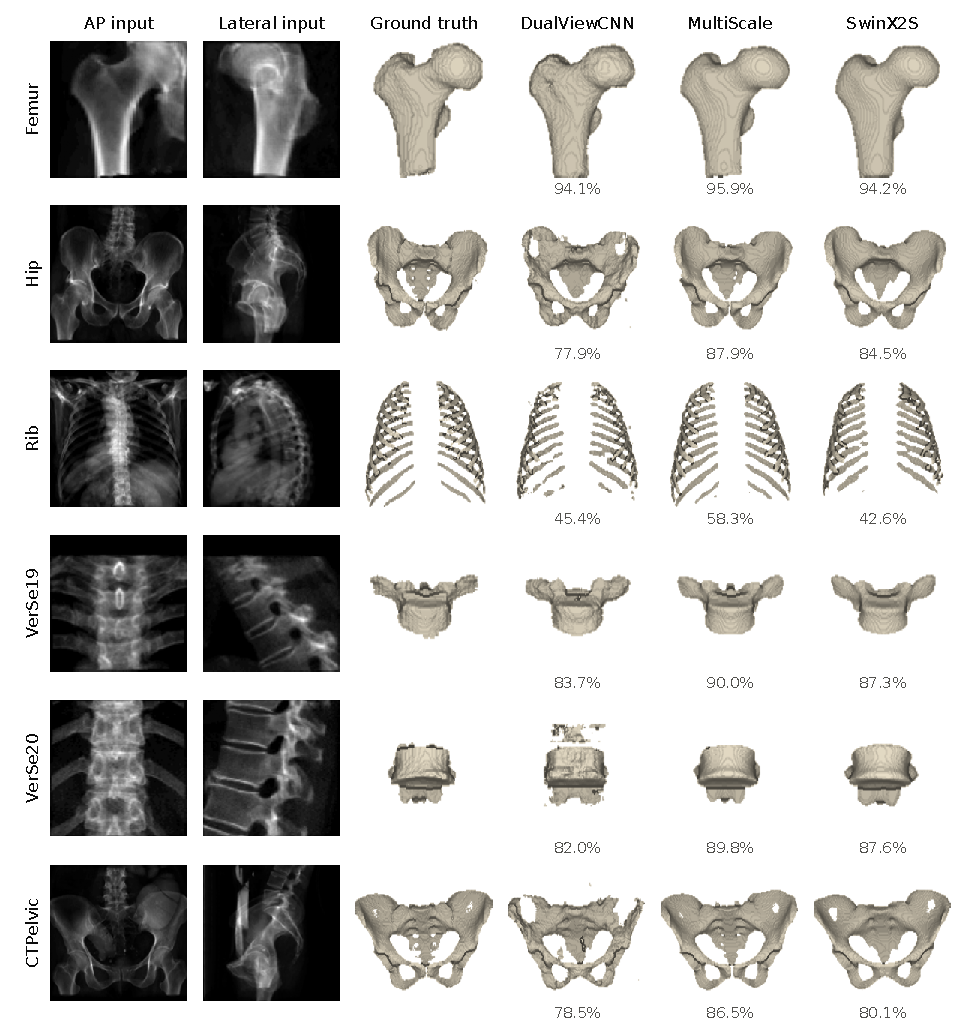
\includegraphics[width=0.92\textwidth]{figures/qualitative.pdf}
\caption{Typical test cases. For each dataset we show a case whose MultiScale Dice is close to the median MultiScale test Dice. All panels show the same square region around the bone. The AP image is shown as given to the models, that is, mirrored to match the volume (Section~\ref{sec:problem}). The 3D shapes are shaded surfaces seen from the front, with the same left--right orientation as the AP image. Percentages are each model's Dice on that case.}
\label{fig:qual}
\end{figure}

The rib cage is hard for all three models. MultiScale reaches 56.4\% Dice, and the other two stay below 48\%, with mean HD95 values of 20.6\,mm (DualViewCNN) and 28.2\,mm (SwinX2S) against 9.0\,mm for MultiScale. Fig.~\ref{fig:qual} shows that MultiScale gets the overall shape of the rib cage but not every single thin rib. With 2.5\,mm voxels a rib is only a few voxels thick, and the ribs overlap each other in both images.

\subsection{Training behaviour}
Fig.~\ref{fig:curves} shows the validation Dice during training. All 18 runs improve steadily and end within 0.9 points of their best validation Dice. Eleven runs stopped early after 40 epochs without improvement, five reached the epoch limit, and the two SwinX2S runs on hip and CTPelvic stopped at the time limit (Section~\ref{sec:setup}). The chosen checkpoints come from epochs 107 to 200. SwinX2S reaches its best validation Dice late in training (epochs 113 to 196), and its precision and recall stay close (Table~\ref{tab:metrics}). Fig.~\ref{fig:loss} shows the training and validation losses of three runs.

\begin{figure}[t]
\centering
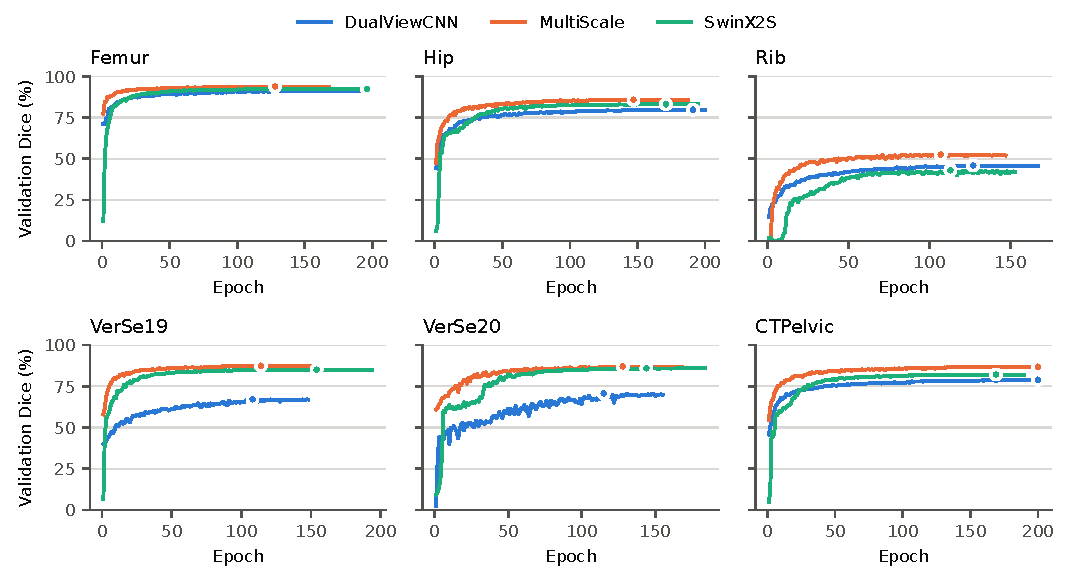
\includegraphics[width=\textwidth]{figures/validation_curves.pdf}
\caption{Validation Dice during training for all 18 runs. Dots mark the chosen checkpoints. Runs end at the epoch limit, by early stopping, or (SwinX2S on hip and CTPelvic) at the time limit of the cloud GPUs.}
\label{fig:curves}
\end{figure}

\begin{figure}[t]
\centering
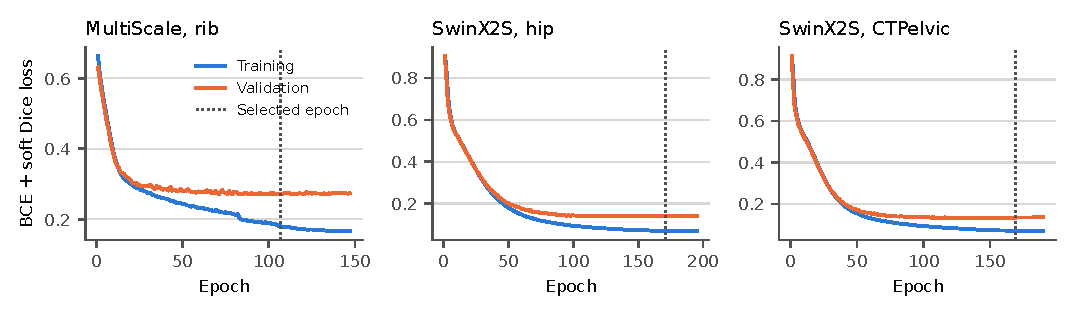
\includegraphics[width=\textwidth]{figures/loss_curves.pdf}
\caption{Training and validation loss for three runs. Dotted lines mark the chosen epoch (best validation Dice). Training losses are computed on augmented samples.}
\label{fig:loss}
\end{figure}

For all three model types, some epochs recorded a non-finite mean gradient norm (Appendix~\ref{app:training}, Table~\ref{tab:stability}): between 0 and 27 epochs per run. This is most likely overflow in mixed precision. When it happens, the gradient scaler skips the step and lowers its scale factor. The losses and validation scores always stayed finite. The runs with many optimizer steps (femur and VerSe19, 16 to 27 epochs) had the most such epochs and the VerSe20 runs, with the fewest steps, the fewest (0 to 3), as expected when the scaler regularly tries a larger scale factor. It therefore reflects normal mixed-precision training, not instability.

\subsection{Model size}
MultiScale has 3.73 million parameters, 8.7 times fewer than SwinX2S (32.5 million). DualViewCNN is the smallest (0.56 million; 1.26 million on rib). We did not measure inference time or memory use, because the training runs used different GPUs and often shared a GPU with other jobs.

% ======================================================================
\section{Discussion}\label{sec:discussion}

\subsection{What the results show}
With both views placed according to the X-ray geometry and with the same epoch limit, batch size and early stopping, the same model came first on all six datasets. The gap between MultiScale and SwinX2S is small on femur, the vertebrae and hip (0.9 to 2.7 points) and larger on CTPelvic (4.1) and rib (11.0). DualViewCNN is close on femur but far behind on the vertebrae. These are results for three specific implementations trained once with the settings in Table~\ref{tab:training}. The rest of this section discusses possible reasons. We did not test any of them with a controlled experiment.

\subsection{Model size, amount of data and training}
SwinX2S has 8.7 times more parameters than MultiScale but was trained on only 85 to 747 samples, from scratch, without the pretrained weights that Swin models usually start from~\cite{swin2021}. Transformers usually need large training sets or pretraining to match CNNs~\cite{dosovitskiy2021}. The cross-view block has no residual connection (as in the official code), so the bottleneck features of each view are replaced by features taken from the other view. We also kept each model's own optimizer and learning rate without tuning them, so a model whose default setting suits our data less well is at a disadvantage. A comparison with tuned learning rates, several seeds, pretrained weights and larger training sets would show whether the remaining gap between MultiScale and SwinX2S comes from the architecture.

\subsection{Differences between anatomies}
Femur and vertebrae were reconstructed best, the two pelvis datasets next, and the rib cage worst. Neither Dice nor the surface metrics can be compared directly across anatomies, because structure size, box size, voxel size and cutting by the box differ between datasets. Hip and CTPelvic have the same target (both hip bones and the sacrum), and MultiScale reached almost the same Dice on both (87.0\% and 86.6\%), even though the CT collections are different. The rib cage is hard for several reasons. The ribs are thin and curved and overlap in both images, the output grid is coarse compared with the thickness of a rib, and the box often cuts the rib cage. Better rib results probably need finer grids, losses or metrics made for thin structures, or a different way of representing the target.

\subsection{Overlap scores and clinical measurements}\label{sec:clinical}
Clinicians use a bone model to measure values such as femoral length, femoral head diameter, the neck--shaft angle, the orientation of the hip socket (acetabulum) or vertebral height. A high Dice score does not mean that these values are correct~\cite{taha2015,maierhein2024}. Most voxels of a bone lie inside it, so errors at joint surfaces or landmarks change Dice very little, even though these are the places where clinical measurements are taken. A shape that is slightly shifted, rotated or thinned can keep a high Dice while an angle or length measured on it is wrong, and Dice does not show where the error is. Our best femur model reaches 94.9\% Dice with a mean HD95 of 2.4\,mm, so some surface points are several millimetres from the true surface. Whether this matters depends on where these errors are and on which value is measured. We did not measure clinical values for the models in this paper, so our results show how well the shapes match, not clinical accuracy. Also, the femur boxes contain only the upper femur, so values such as total femoral length cannot be measured on these data at all.

% ======================================================================
\section{Limitations and Future Work}\label{sec:limitations}

\paragraph{Simulated X-ray images only.}
All inputs are DRRs made from the same CT region that defines the target. They use a simple intensity model (Equation~\ref{eq:drr}) and have no scatter, noise, changes in patient position or overlapping anatomy from outside the box. We did not test on real X-ray images, so we do not know how the models perform on clinical images.

\paragraph{Splits and independence of cases.}
The splits are made by sample. Vertebrae from the same VerSe scan, and the two femurs of one TotalSegmentator scan, can end up in different splits. This can make the femur and VerSe results too optimistic. In CTPelvic we could not check whether different CT colonography IDs belong to the same patient. The VerSe20 test set has only 10 cases. Four training masks in the femur dataset are empty.

\paragraph{Not a fully controlled comparison.}
The models share the epoch limit, batch size, early stopping, augmentation, loss and view geometry, but they differ in architecture, optimizer, learning rate, schedule and normalization, and the learning rates were not tuned. Each model was trained once with one seed. Two SwinX2S runs stopped at a time limit a few epochs before the epoch limit, at a learning rate near zero, and DualViewCNN and MultiScale on CTPelvic had their best validation Dice at the epoch limit itself, so they might have improved with longer training. Our version of SwinX2S differs from the official code in how the lateral view is arranged for our image layout and in its settings (Tiny model, one attention layer, no pretraining). The results therefore cannot isolate the effect of multi-scale fusion, attention or model size, and they do not include run-to-run variation.

\paragraph{Evaluation.}
Metrics are computed on resampled grids with voxels of 0.75 to 2.5\,mm, so errors smaller than about one voxel cannot be measured. We did not evaluate clinical values, results on abnormal or diseased bones, or computing cost.

\paragraph{Future work.}
These experiments would address the limitations above:
\begin{itemize}
\item tune the learning rate of each model on the validation data, train with several seeds, and test Swin-X2S with pretrained weights, to separate the effect of the architecture from that of the training settings;
\item rebuild the splits by subject using the original scan IDs, and use a new test split;
\item test on real biplanar X-ray images with matching CT, and study how to adapt models trained on DRRs to real images;
\item measure clinical values on the reconstructed bones and compare them with the same measurements on CT;
\item test on abnormal cases and at higher output resolution, especially for the rib cage.
\end{itemize}

% ======================================================================
\section{Conclusion}
We trained and tested three models that reconstruct bone masks from two simulated X-ray images, on six datasets with one pipeline, with both views placed according to the X-ray geometry and the same training budget. A multi-scale network that copies the features of both views into the volume at four resolutions had the highest Dice and the lowest surface errors on every dataset, with far fewer parameters than the transformer model, which came second on five datasets. The rib cage stayed hard for all models. Tests on real X-ray images, splits by subject and direct measurement of clinical values are needed before any clinical use can be considered.

% ======================================================================
\section*{Code and Data Availability}
The 18 trained models, the model and configuration code, and a list of the model files will be available at \url{https://huggingface.co/jeevan1234/biplanar-bone-reconstruction-models}. The ancillary files of this arXiv submission contain the split lists, the training logs, the per-case validation and test results, the geometry and projection tests, and the scripts that make the tables and figures. A README in the ancillary folder lists them. The image data behind the example figures are not included, because they are derived from the datasets. The code, data splits and per-case results are available at \url{https://github.com/Jeevan-Neupane/biplanar-bone-reconstruction} (release v1.0). The SwinX2S code is adapted from the official Swin-X2S repository (\url{https://github.com/liukuan5625/Swin-X2S}, MIT licence). NAAMII provided the processed datasets. They are derived from TotalSegmentator (CC BY 4.0), VerSe (CC BY-SA 4.0) and CTPelvic1K (CC BY-NC-SA), are not shared with this paper, and remain under those licences.

\section*{Ethics}
This study used only public, de-identified CT datasets released for research. We did not collect any new data from people.

\section*{Acknowledgements}
We thank the Nepal Applied Mathematics and Informatics Institute for Research (NAAMII) for providing the processed datasets, for building and sharing the open-source XrayTo3DPreprocess pipeline used to make them, and for its support and guidance throughout this work. We also thank the Department of Electronics and Computer Engineering, Pulchowk Campus, for supporting the project this work is based on, and the creators of TotalSegmentator, VerSe and CTPelvic1K for making their data public.

\FloatBarrier
\bibliographystyle{unsrtnat}
\bibliography{references}

% ======================================================================
\appendix
\FloatBarrier
\section{A C++ DRR Renderer}\label{app:renderer}
We also built a CT-to-DRR renderer in C++ (Fig.~\ref{fig:drr}), based on the open-source DRR-renderer of Habert~\cite{habert2017drr}. It reads CT scans in MetaImage or NIfTI format. It uses the voxel size and direction matrix in the file header, and for NIfTI files also the origin, to place the scan in world coordinates in millimetres. A point source is placed 4000\,mm from the centre of the scan, and a $1024\times1024$ detector with 1\,mm pixels is placed 2000\,mm from the centre on the other side. For the AP view the source is in front of the patient, and for the lateral view it is at the patient's side. For each detector pixel, the ray from the source is clipped to the scan and sampled at steps equal to the smallest voxel size, with trilinear interpolation of the CT values. A CT value $h$ is converted to $\mu=\mu_w(1+h/1000)$ with $\mu_w=0.022\,\mathrm{mm}^{-1}$ if $h>200$\,HU, and to zero otherwise, so that mainly bone is visible. The pixel value is the mean of $\mu$ along the ray, a simplified form of the Beer--Lambert line integral. Each image is scaled to $[0,1]$ and saved as an 8-bit PNG. Compared with the original renderer, we added NIfTI support, the full mapping to world coordinates, the fixed AP and lateral setup, the bone threshold and the larger detector. The models in this paper were trained and tested on the NAAMII DRRs (Section~\ref{sec:drr}), not on images from this renderer. The source code is in the project repository.

\begin{figure}[H]
\centering
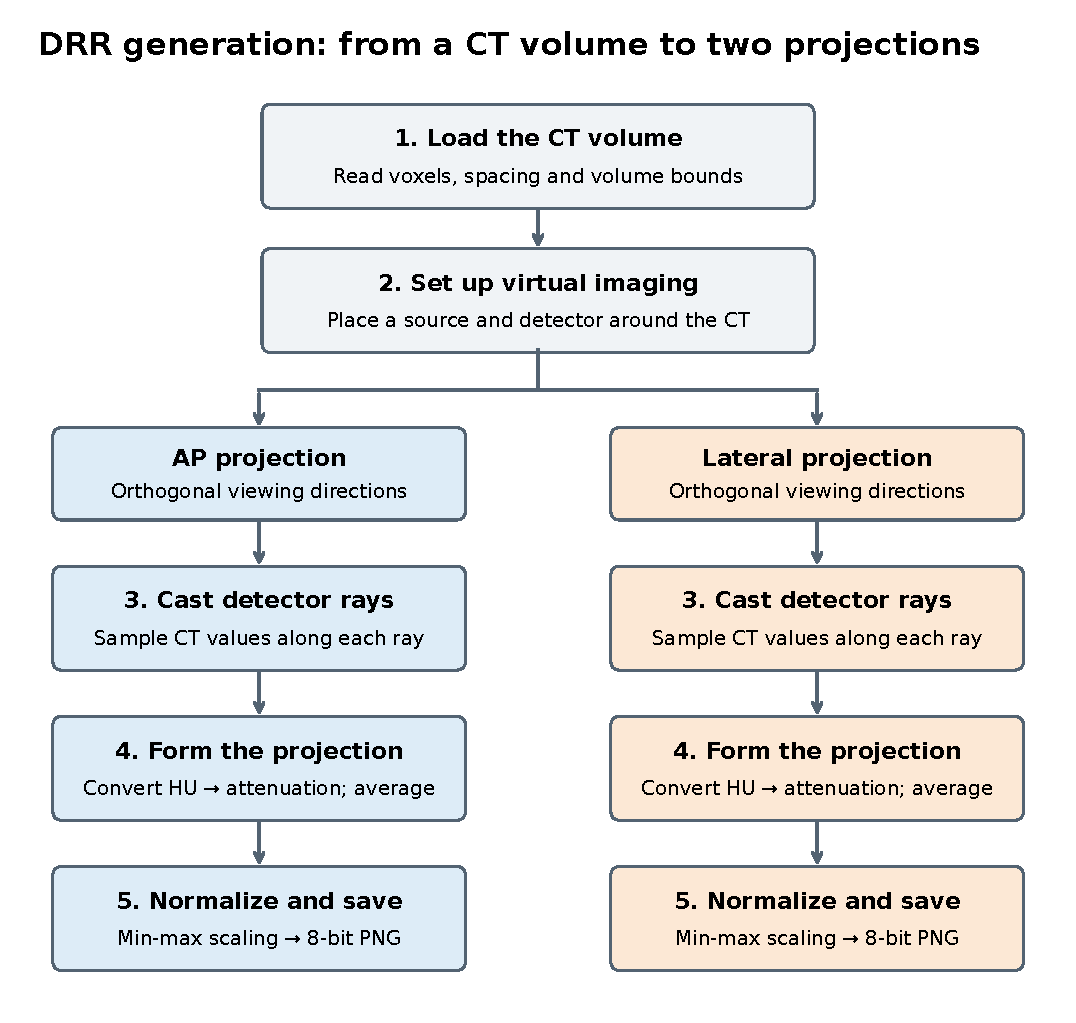
\includegraphics[width=0.55\textwidth]{figures/drr_generation.pdf}
\caption{Steps of the C++ DRR renderer. Each ray is clipped to the CT scan and sampled. CT values are turned into attenuation values (zero at or below 200\,HU) and averaged along the ray, and the image is saved as an 8-bit PNG.}
\label{fig:drr}
\end{figure}

\section{Validation Results and Training Details}\label{app:training}
Table~\ref{tab:val} gives the validation scores of each chosen checkpoint, and Table~\ref{tab:stability} summarizes each training run.

\begin{table}[H]
\centering
\caption{Validation scores (\%) of the chosen checkpoint of each run, with its epoch and validation loss.}
\label{tab:val}
\small
\begin{tabular}{llrrrrrr}
\toprule
Dataset & Model & Epoch & Dice & IoU & Prec. & Rec. & Loss \\
\midrule
Femur & DualViewCNN & 197 & 91.3 & 85.3 & 90.7 & 92.3 & 0.071 \\
 & MultiScale & 128 & 93.8 & 89.5 & 93.5 & 94.2 & 0.055 \\
 & SwinX2S & 196 & 92.4 & 86.9 & 92.5 & 92.5 & 0.078 \\
Hip & DualViewCNN & 191 & 79.7 & 66.7 & 78.3 & 81.3 & 0.139 \\
 & MultiScale & 147 & 85.7 & 75.4 & 84.6 & 86.9 & 0.104 \\
 & SwinX2S & 171 & 83.0 & 71.3 & 81.7 & 84.5 & 0.139 \\
Rib & DualViewCNN & 127 & 45.8 & 30.4 & 42.4 & 50.4 & 0.306 \\
 & MultiScale & 107 & 52.5 & 36.4 & 49.7 & 56.0 & 0.270 \\
 & SwinX2S & 113 & 43.0 & 28.1 & 43.4 & 43.5 & 0.353 \\
VerSe19 & DualViewCNN & 108 & 67.2 & 52.8 & 65.6 & 69.5 & 0.221 \\
 & MultiScale & 114 & 87.5 & 78.4 & 87.2 & 87.9 & 0.088 \\
 & SwinX2S & 154 & 85.1 & 74.9 & 85.3 & 85.2 & 0.121 \\
VerSe20 & DualViewCNN & 115 & 70.7 & 55.8 & 71.9 & 69.8 & 0.214 \\
 & MultiScale & 128 & 87.1 & 77.6 & 87.5 & 87.0 & 0.098 \\
 & SwinX2S & 144 & 85.9 & 75.5 & 86.1 & 86.1 & 0.196 \\
CTPelvic & DualViewCNN & 200 & 79.0 & 65.5 & 76.8 & 81.4 & 0.138 \\
 & MultiScale & 200 & 86.8 & 76.9 & 86.2 & 87.6 & 0.090 \\
 & SwinX2S & 169 & 82.2 & 69.9 & 80.7 & 83.8 & 0.135 \\
\bottomrule
\end{tabular}

\end{table}

\begin{table}[H]
\centering
\caption{Epochs trained out of the epoch limit, validation Dice (\%) and losses at the last epoch, and the number of epochs with a non-finite mean gradient norm. SwinX2S on hip (195 epochs) and CTPelvic (190) stopped at the time limit of the cloud GPUs.}
\label{tab:stability}
\small
\begin{tabular}{llrrrrr}
\toprule
Dataset & Model & Epochs & Final Dice & Train loss & Val.\ loss & Non-finite \\
\midrule
Femur & DualViewCNN & 200/200 & 91.2 & 0.055 & 0.072 & 20 \\
 & MultiScale & 168/200 & 93.8 & 0.031 & 0.056 & 16 \\
 & SwinX2S & 200/200 & 92.4 & 0.040 & 0.078 & 19 \\
Hip & DualViewCNN & 200/200 & 79.7 & 0.118 & 0.139 & 11 \\
 & MultiScale & 187/200 & 85.7 & 0.055 & 0.104 & 8 \\
 & SwinX2S & 195/200 & 82.9 & 0.068 & 0.140 & 8 \\
Rib & DualViewCNN & 167/200 & 45.8 & 0.266 & 0.306 & 9 \\
 & MultiScale & 147/200 & 51.9 & 0.166 & 0.274 & 9 \\
 & SwinX2S & 153/200 & 42.1 & 0.225 & 0.356 & 8 \\
VerSe19 & DualViewCNN & 148/200 & 67.0 & 0.161 & 0.221 & 20 \\
 & MultiScale & 154/200 & 87.4 & 0.054 & 0.088 & 18 \\
 & SwinX2S & 194/200 & 85.0 & 0.055 & 0.123 & 27 \\
VerSe20 & DualViewCNN & 155/200 & 69.8 & 0.146 & 0.218 & 3 \\
 & MultiScale & 168/200 & 86.8 & 0.050 & 0.102 & 0 \\
 & SwinX2S & 184/200 & 85.9 & 0.149 & 0.193 & 1 \\
CTPelvic & DualViewCNN & 200/200 & 79.0 & 0.128 & 0.138 & 15 \\
 & MultiScale & 200/200 & 86.8 & 0.050 & 0.090 & 12 \\
 & SwinX2S & 190/200 & 82.1 & 0.070 & 0.136 & 12 \\
\bottomrule
\end{tabular}

\end{table}

\end{document}
